\begin{figure*}
  \centering
  \begin{tabular}{c c c c c c}
  \begin{sideways}\bf \small \quad\quad $\detroi$\end{sideways}&
  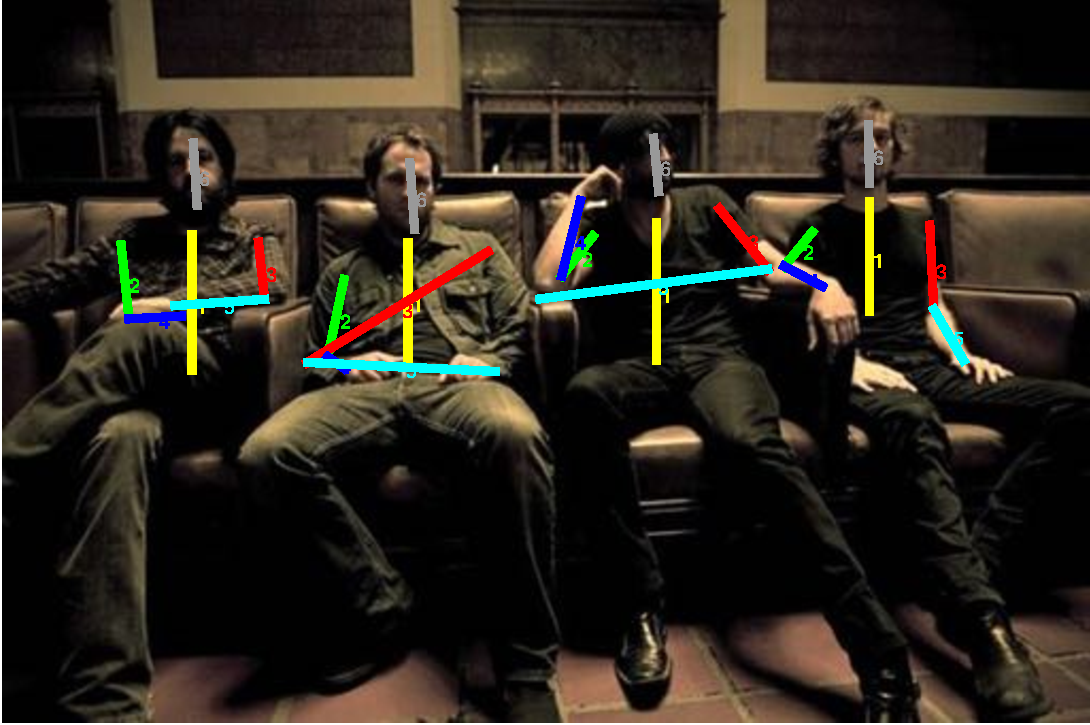
\includegraphics[height=0.150\linewidth]{imgidx_0012_sticks_unary_waf.pdf}&
  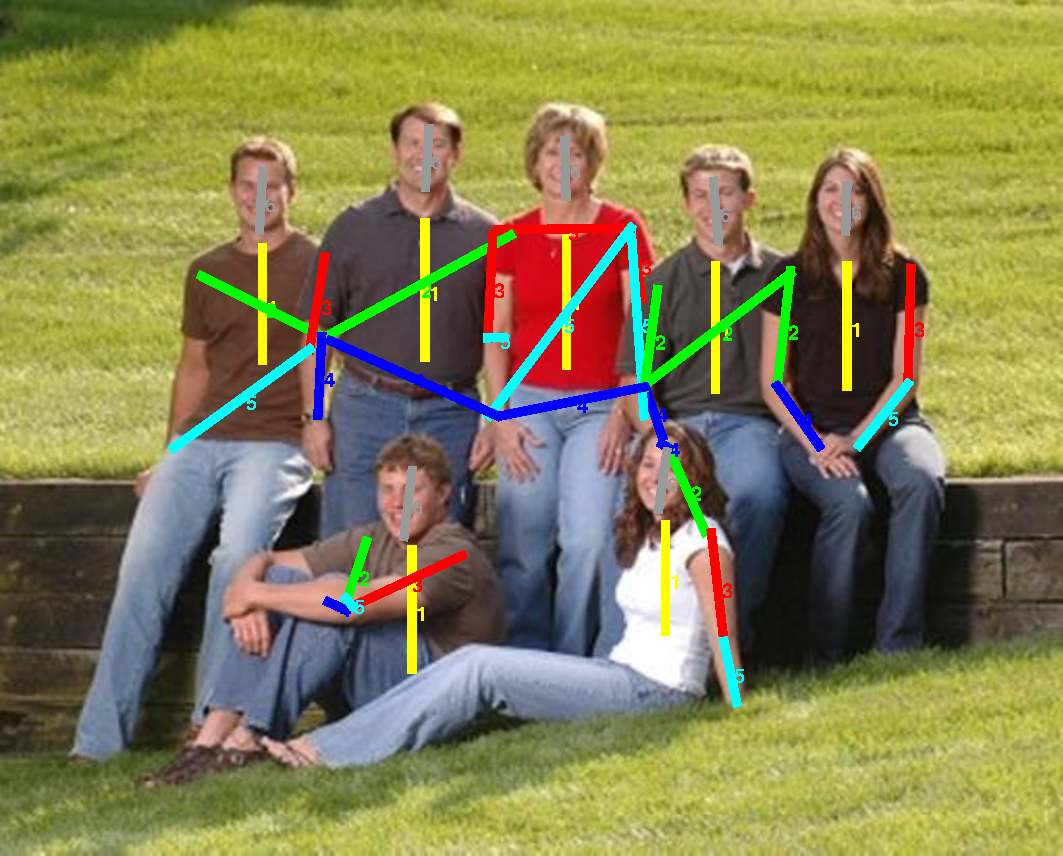
\includegraphics[height=0.150\linewidth]{imgidx_0045_sticks_unary_waf.pdf}&
  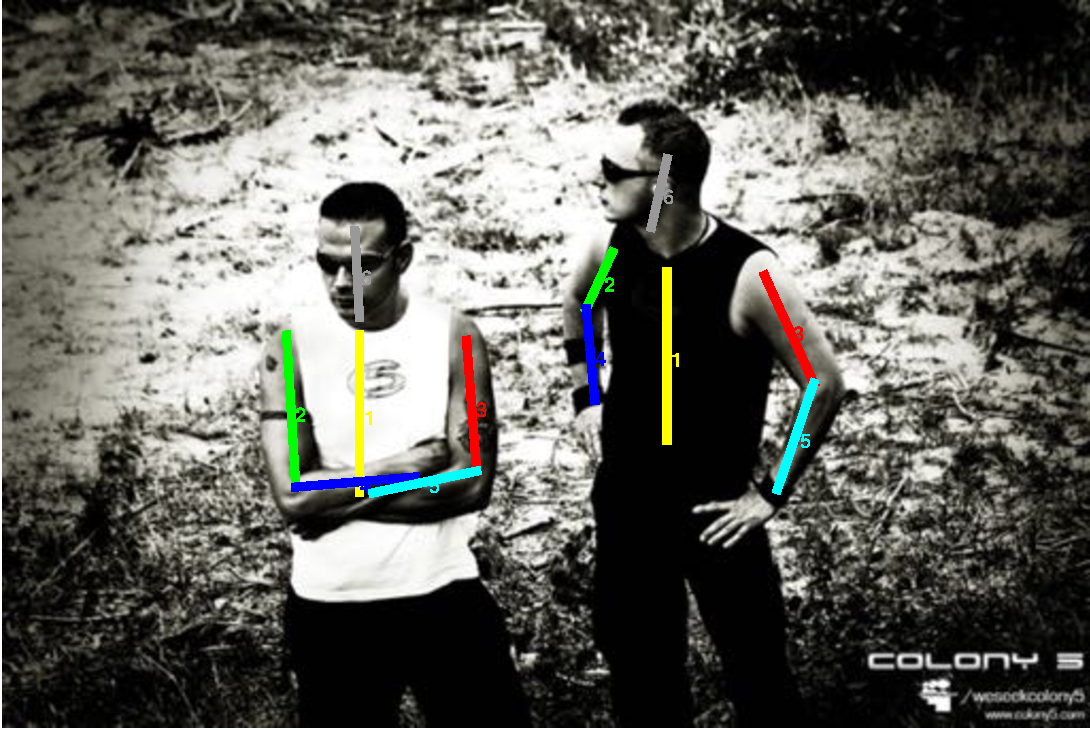
\includegraphics[height=0.150\linewidth]{imgidx_0070_sticks_unary_waf.pdf}&
  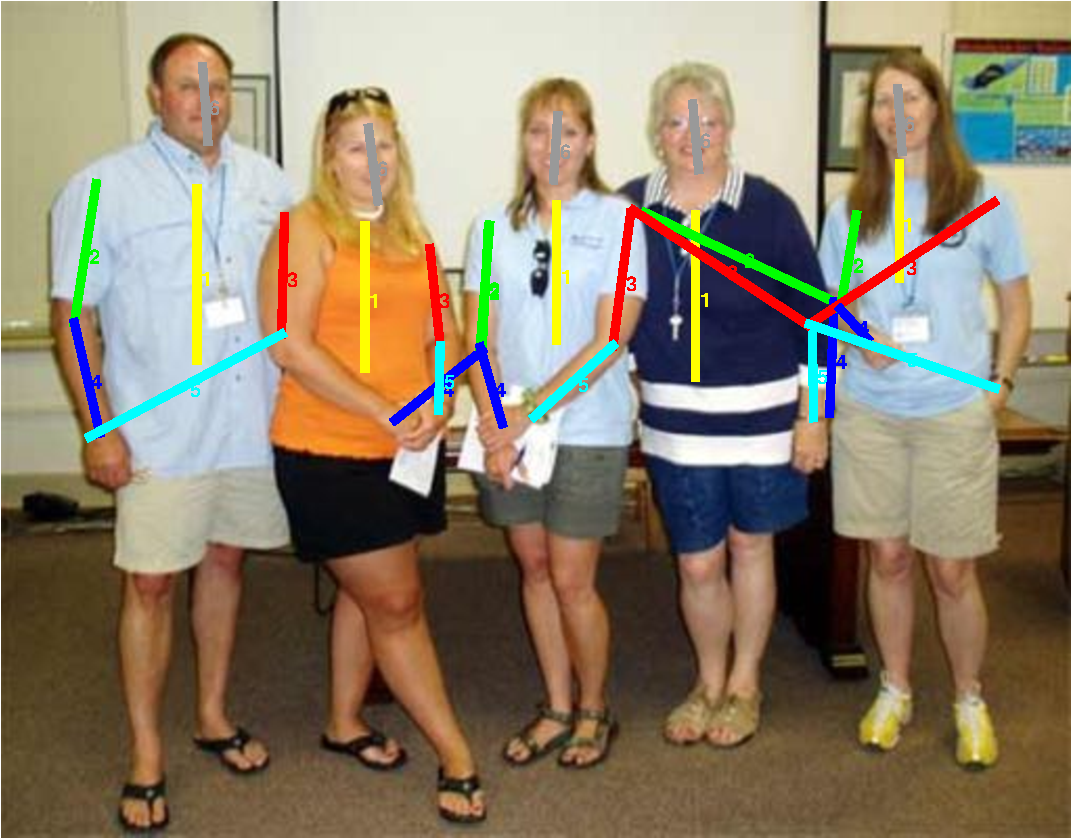
\includegraphics[height=0.150\linewidth]{imgidx_0167_sticks_unary_waf.pdf}&
  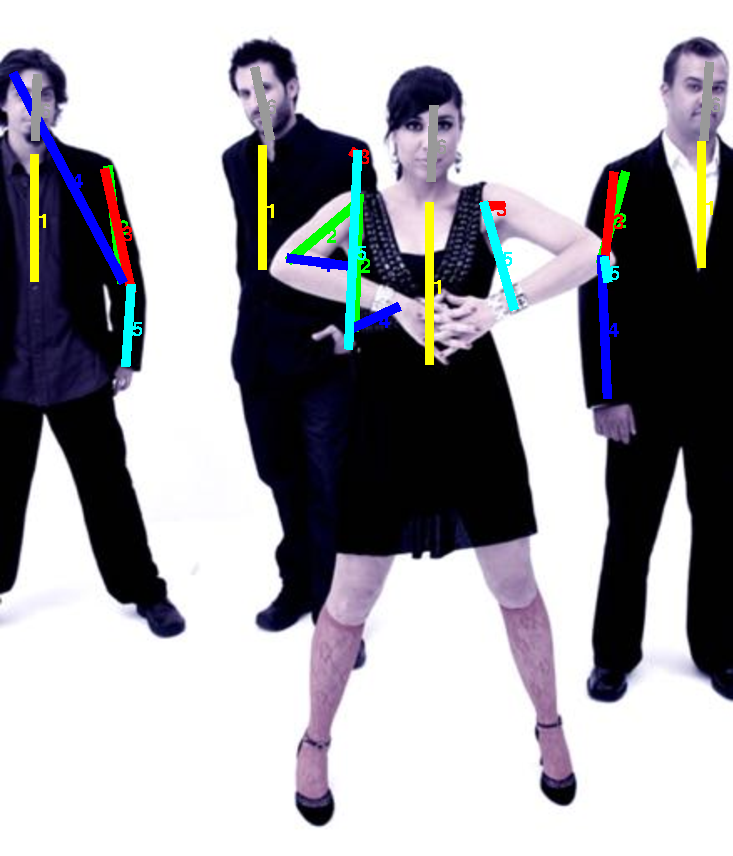
\includegraphics[height=0.150\linewidth]{imgidx_0169_sticks_unary_waf.pdf}\\
  \begin{sideways}\bf \small\quad $\deepcut~\multb$\end{sideways}&
  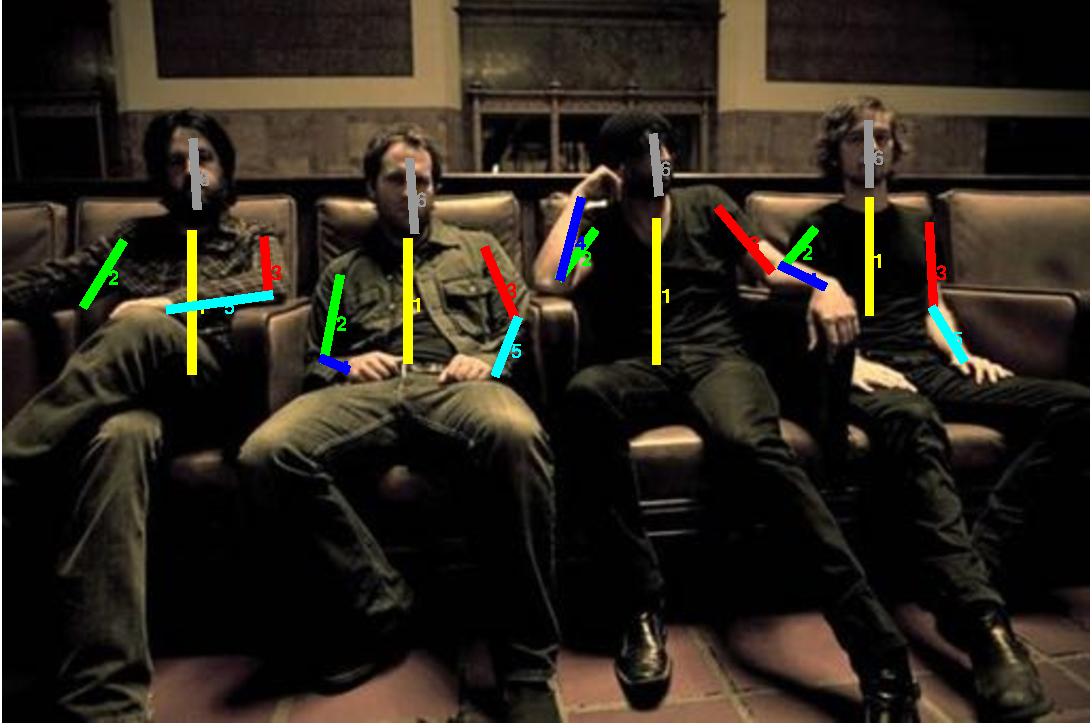
\includegraphics[height=0.150\linewidth]{imgidx_0012_sticks_waf.pdf}&
  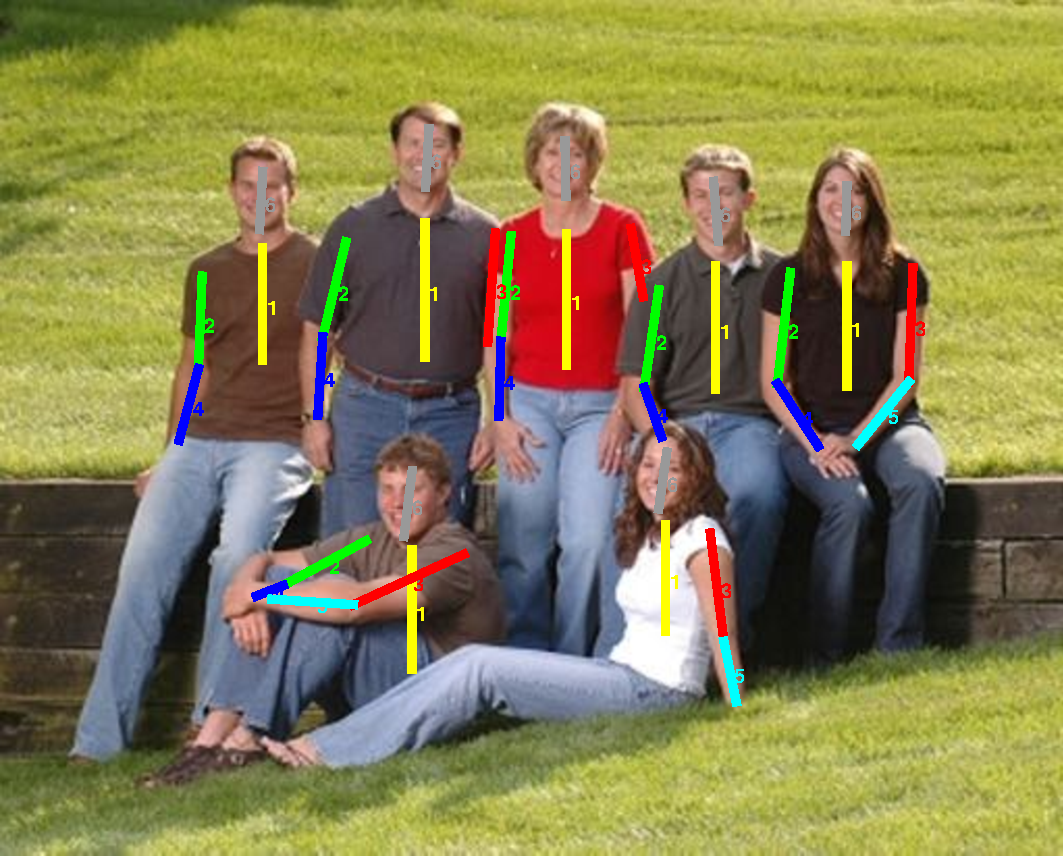
\includegraphics[height=0.150\linewidth]{imgidx_0045_sticks_waf.pdf}&
  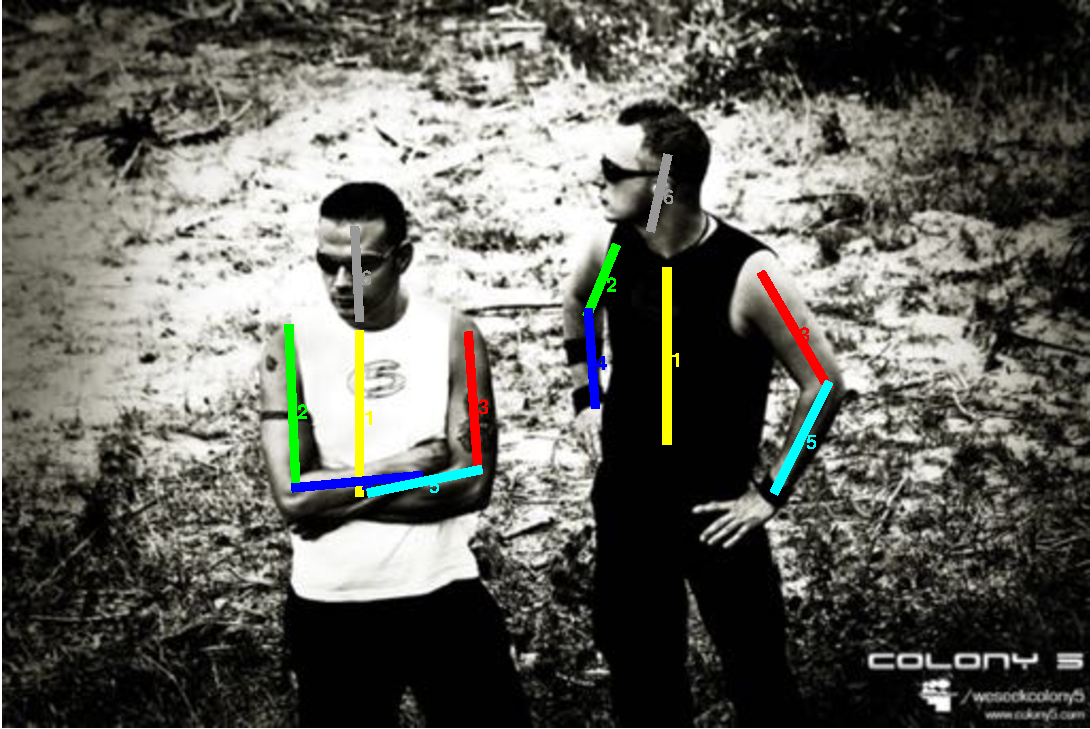
\includegraphics[height=0.150\linewidth]{imgidx_0070_sticks_waf.pdf}&
  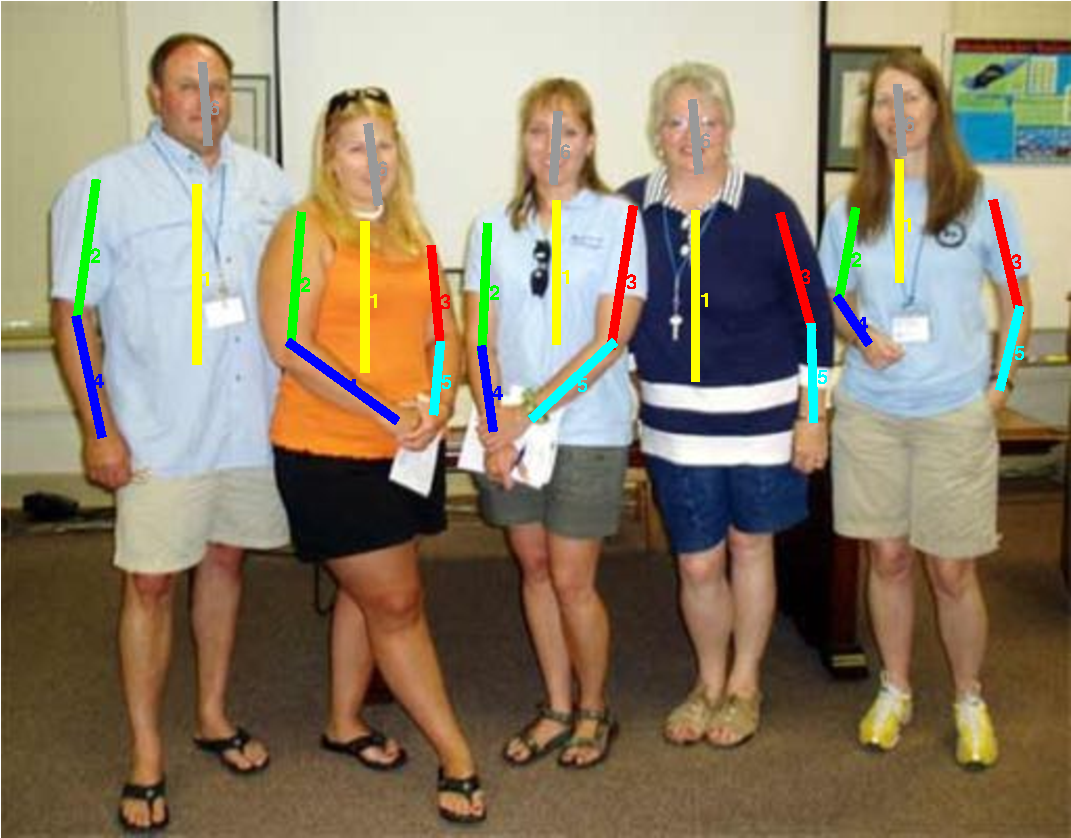
\includegraphics[height=0.150\linewidth]{imgidx_0167_sticks_waf.pdf}&
  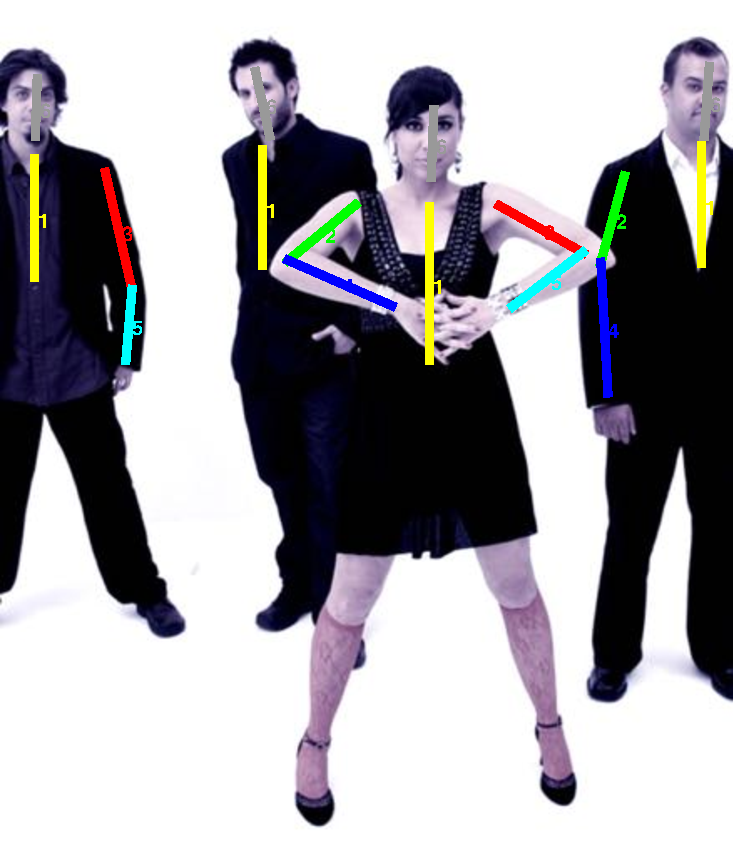
\includegraphics[height=0.150\linewidth]{imgidx_0169_sticks_waf.pdf}\\
  \begin{sideways}\bf \small Chen\&Yuille~\cite{Chen:2015:POC}\end{sideways}&
  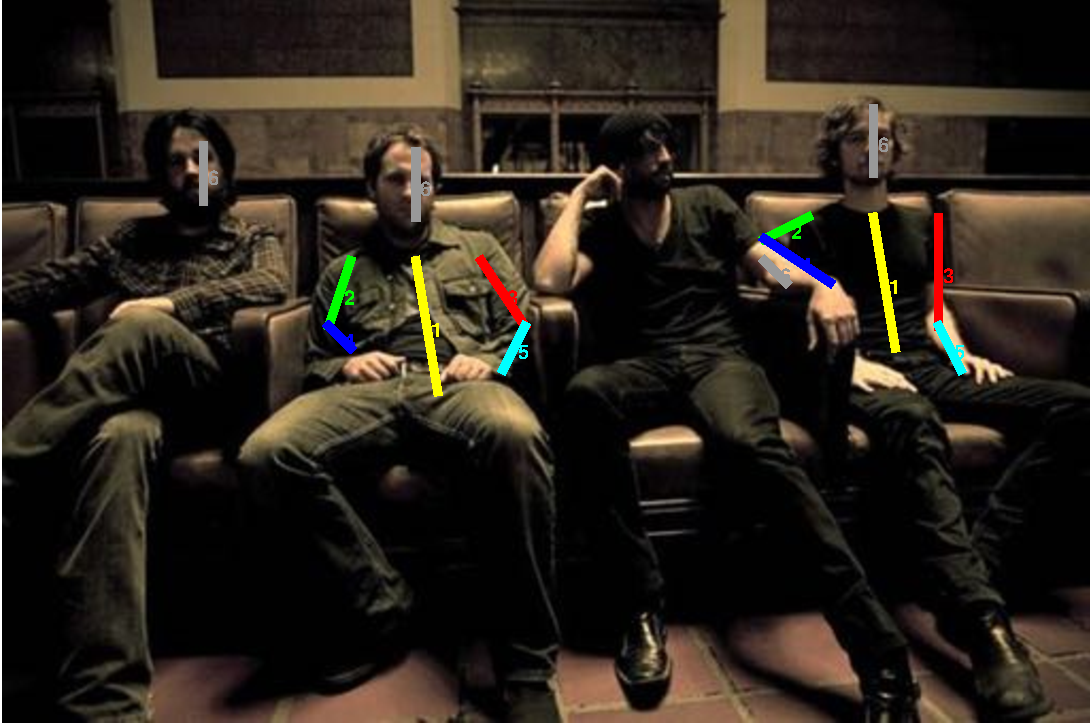
\includegraphics[height=0.150\linewidth]{imgidx_0012_sticks_chen_waf.pdf}&
  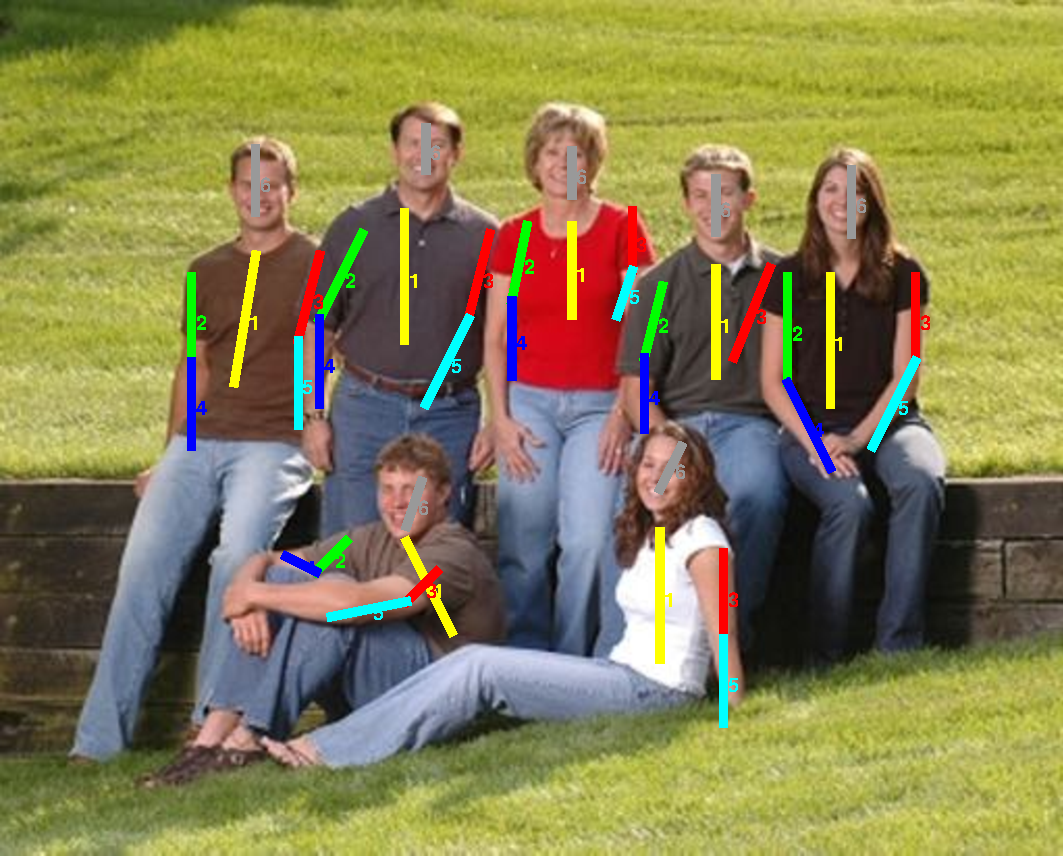
\includegraphics[height=0.150\linewidth]{imgidx_0045_sticks_chen_waf.pdf}&
  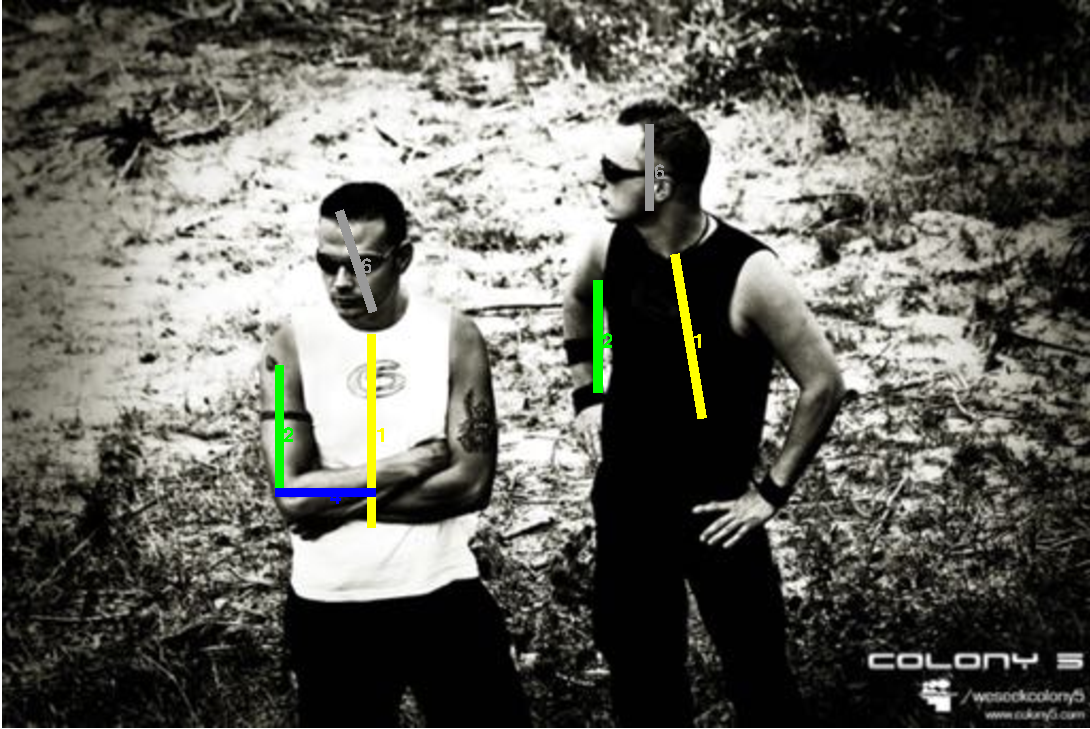
\includegraphics[height=0.150\linewidth]{imgidx_0070_sticks_chen_waf.pdf}&
  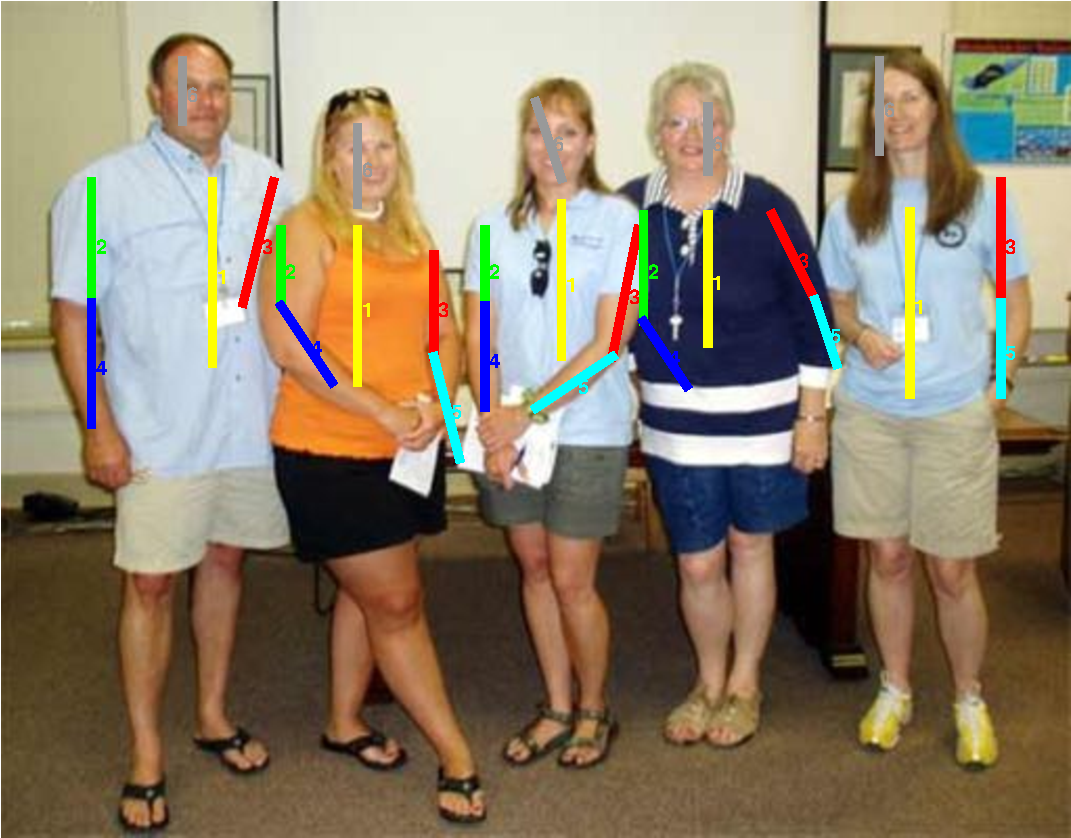
\includegraphics[height=0.150\linewidth]{imgidx_0167_sticks_chen_waf.pdf}&
  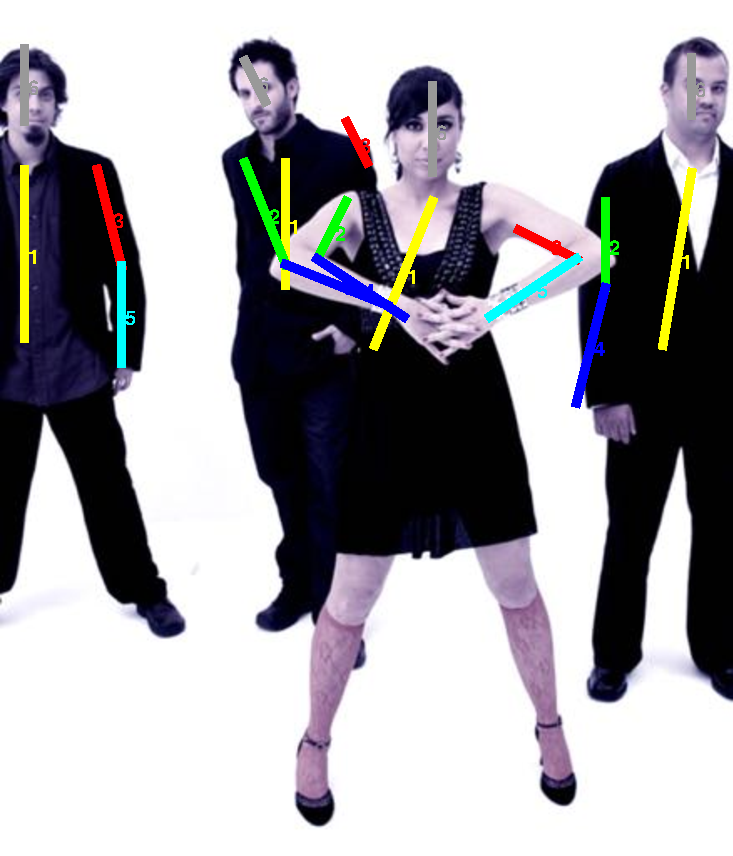
\includegraphics[height=0.150\linewidth]{imgidx_0169_sticks_chen_waf.pdf}\\
  %&1&2&3&4&5\\
 %%  \includegraphics[height=0.275\linewidth]{imgidx_0073_sticks_waf.pdf}&
%%   \includegraphics[height=0.275\linewidth]{imgidx_0073_sticks_unary_waf.pdf}\\
  %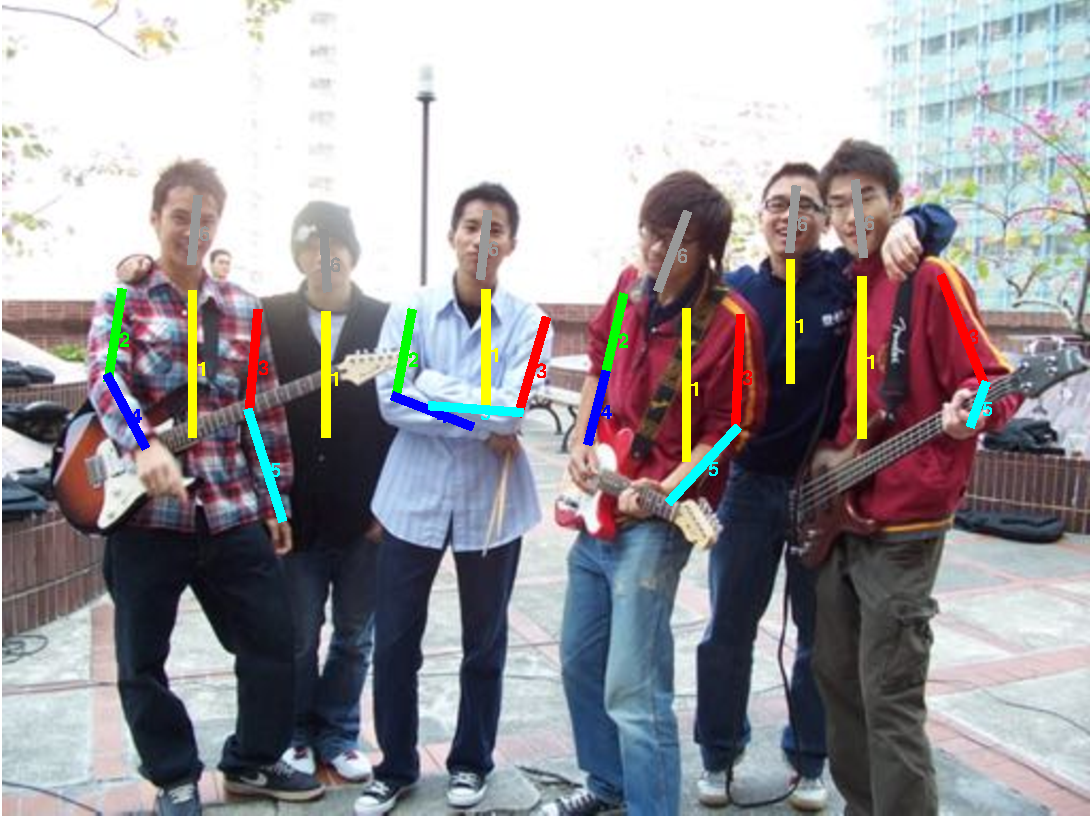
\includegraphics[height=0.275\linewidth]{imgidx_0112_sticks_waf.pdf}&

  %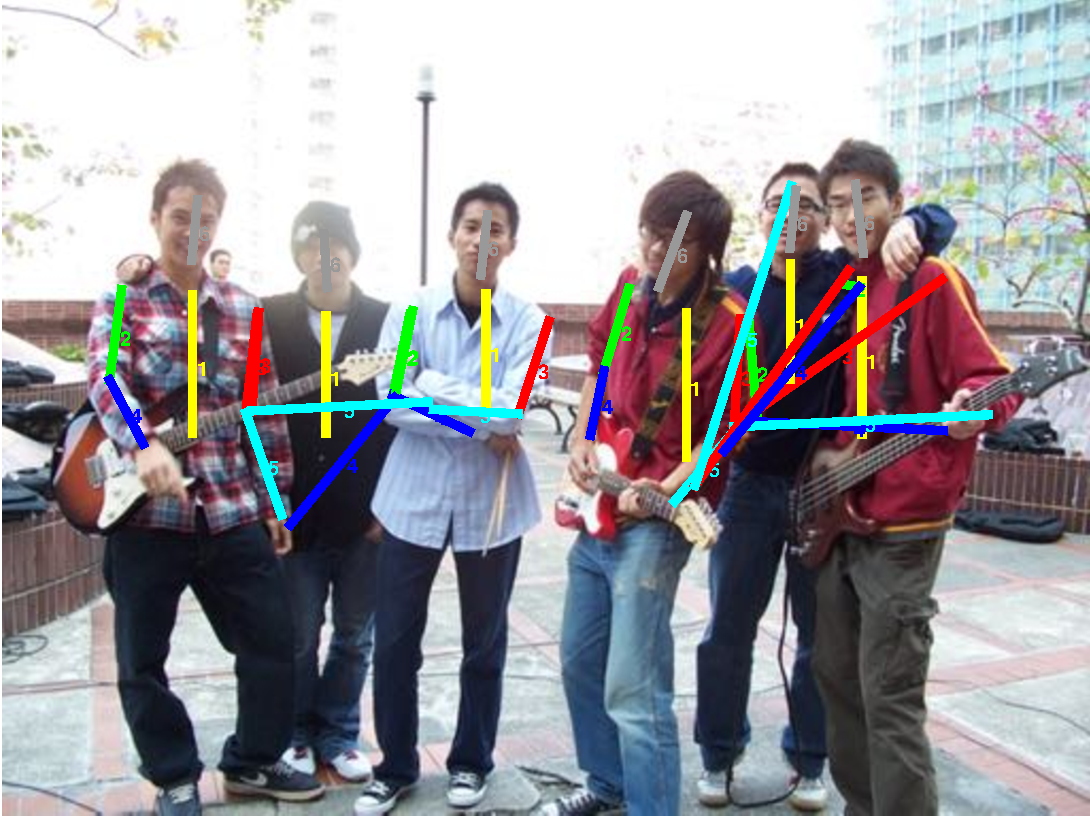
\includegraphics[height=0.275\linewidth]{imgidx_0112_sticks_unary_waf.pdf}\\
%%   \includegraphics[height=0.275\linewidth]{imgidx_0103_sticks_waf.pdf}&
%%   \includegraphics[height=0.275\linewidth]{imgidx_0103_sticks_unary_waf.pdf}\\
  %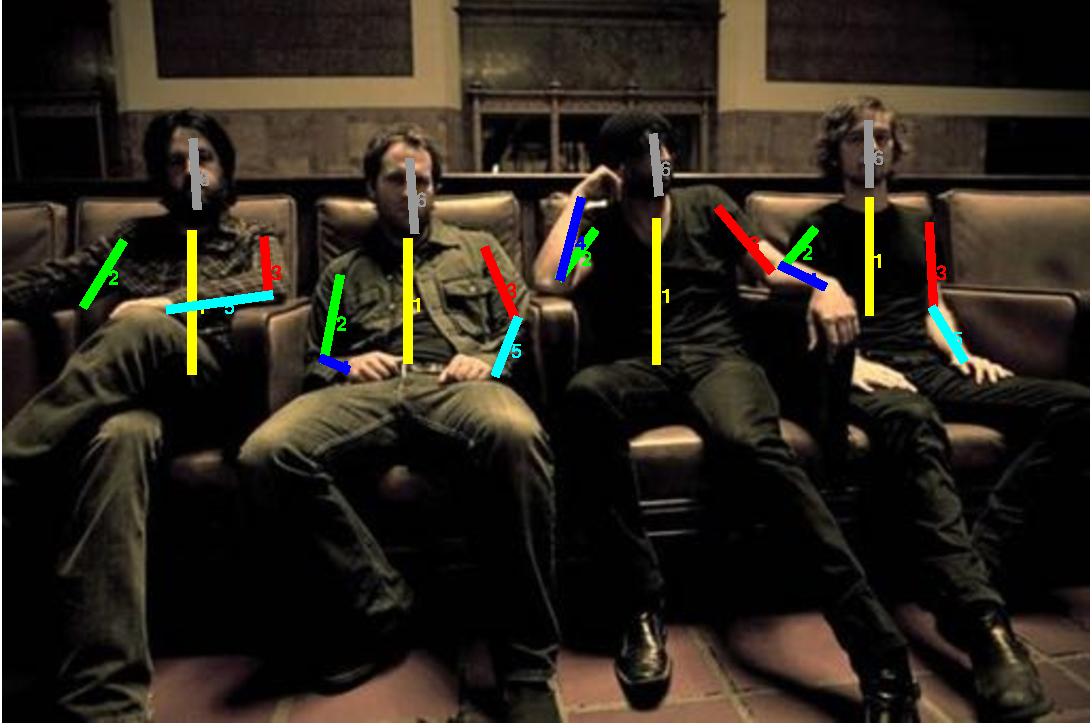
\includegraphics[height=0.275\linewidth]{imgidx_0012_sticks_waf.pdf}&
  %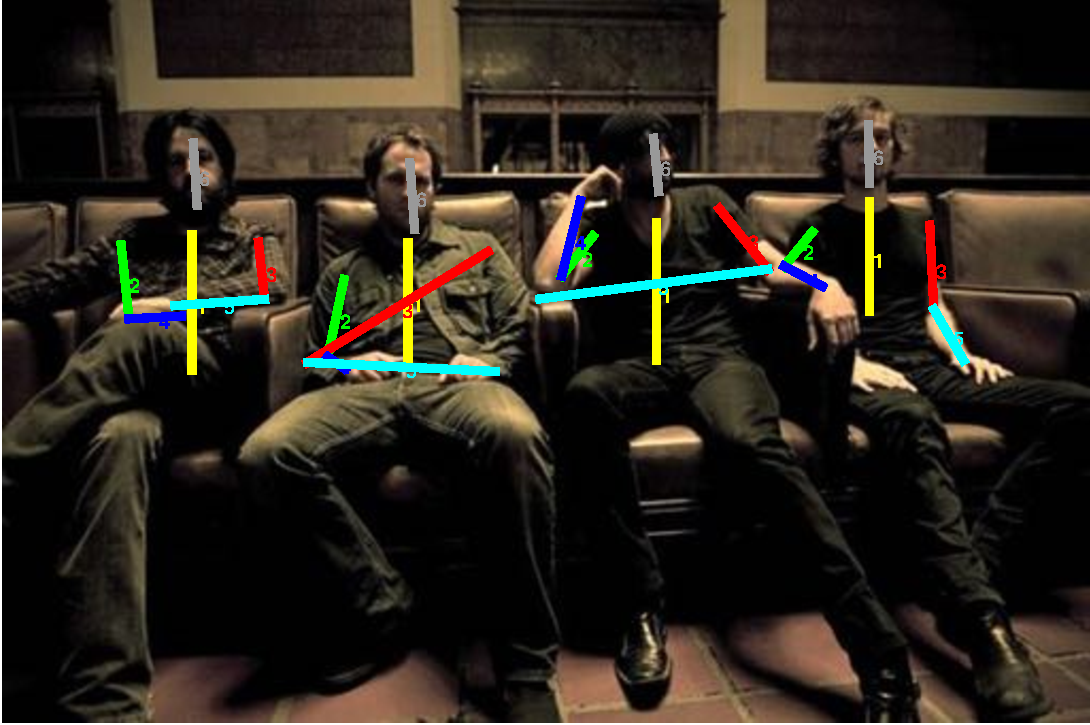
\includegraphics[height=0.275\linewidth]{imgidx_0012_sticks_unary_waf.pdf}\\
%%   \includegraphics[height=0.245\linewidth,width=0.45\linewidth]{imgidx_0026_sticks_waf.pdf}&
%%   \includegraphics[height=0.245\linewidth,width=0.45\linewidth]{imgidx_0026_sticks_unary_waf.pdf}\\
%%   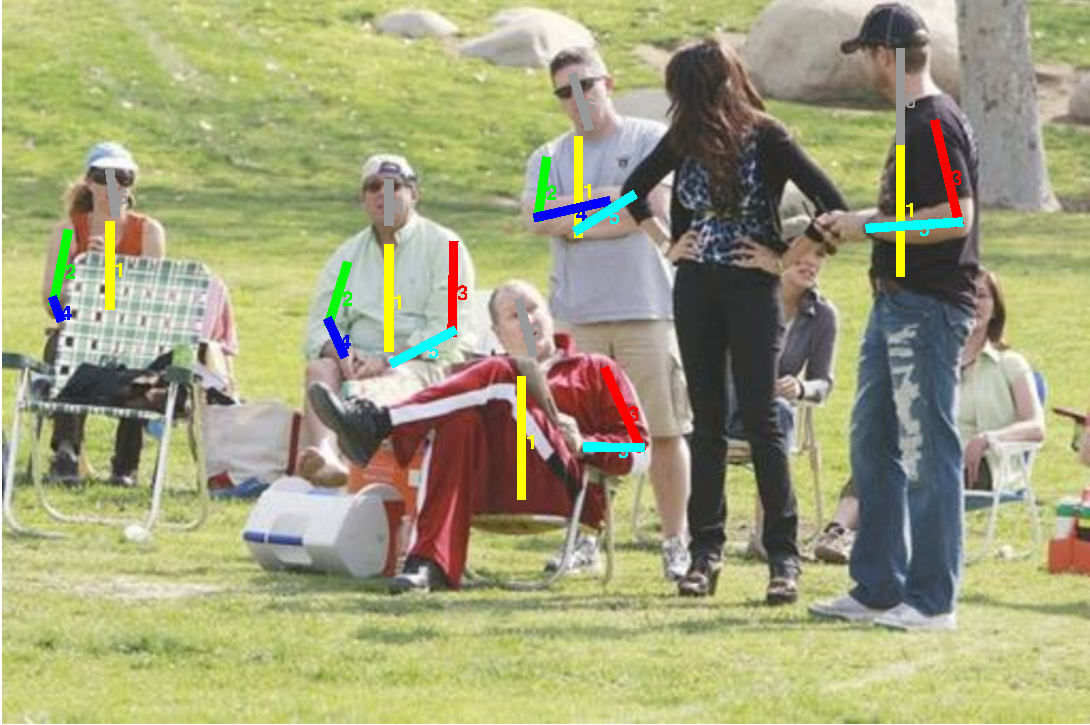
\includegraphics[height=0.245\linewidth,width=0.45\linewidth]{imgidx_0028_sticks_waf.pdf}&
%%   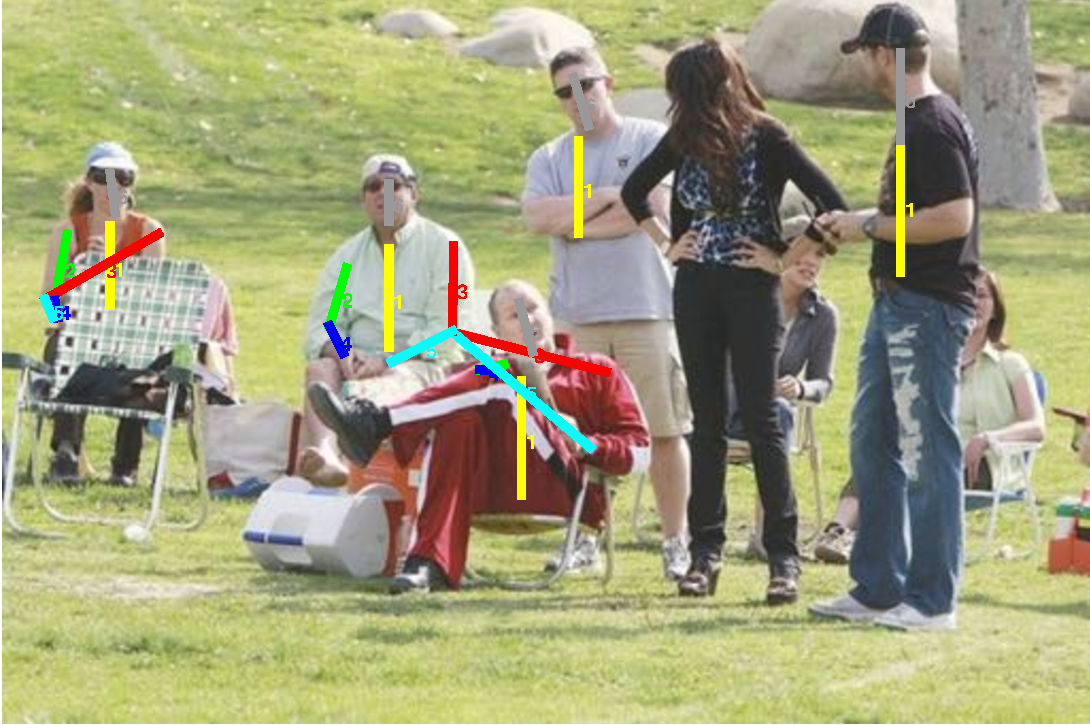
\includegraphics[height=0.245\linewidth,width=0.45\linewidth]{imgidx_0028_sticks_unary_waf.pdf}\\

%%   \includegraphics[height=0.245\linewidth,width=0.45\linewidth]{imgidx_0066_sticks_waf.pdf}&
%%   \includegraphics[height=0.245\linewidth,width=0.45\linewidth]{imgidx_0066_sticks_unary_waf.pdf}\\
%%   \hspace{3.5em}\includegraphics[height=0.275\linewidth]{imgidx_0073_sticks_waf.pdf}&
%%   \hspace{-3.5em}\includegraphics[height=0.275\linewidth]{imgidx_0073_sticks_unary_waf.pdf}\\
%%   \includegraphics[height=0.245\linewidth,width=0.45\linewidth]{imgidx_0104_sticks_waf.pdf}&
%%   \includegraphics[height=0.245\linewidth,width=0.45\linewidth]{imgidx_0104_sticks_unary_waf.pdf}\\

%%   \includegraphics[height=0.245\linewidth,width=0.45\linewidth]{imgidx_0143_sticks_waf.pdf}&
%%   \includegraphics[height=0.245\linewidth,width=0.45\linewidth]{imgidx_0143_sticks_unary_waf.pdf}\\
  %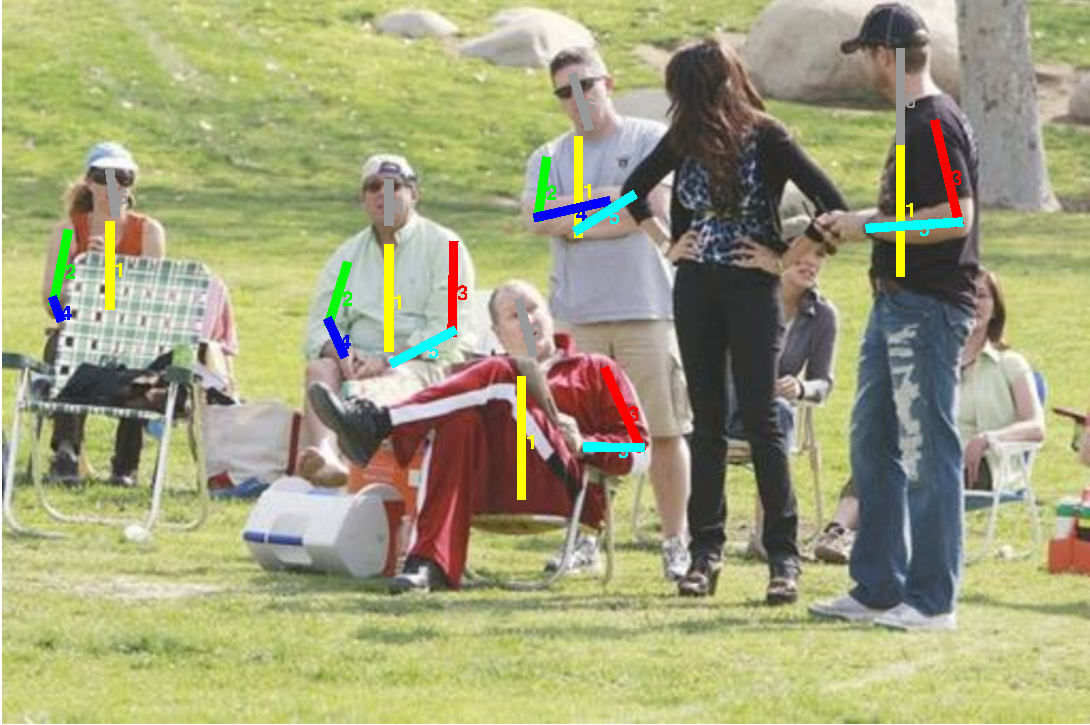
\includegraphics[height=0.275\linewidth]{imgidx_0028_sticks_waf.pdf}&
  %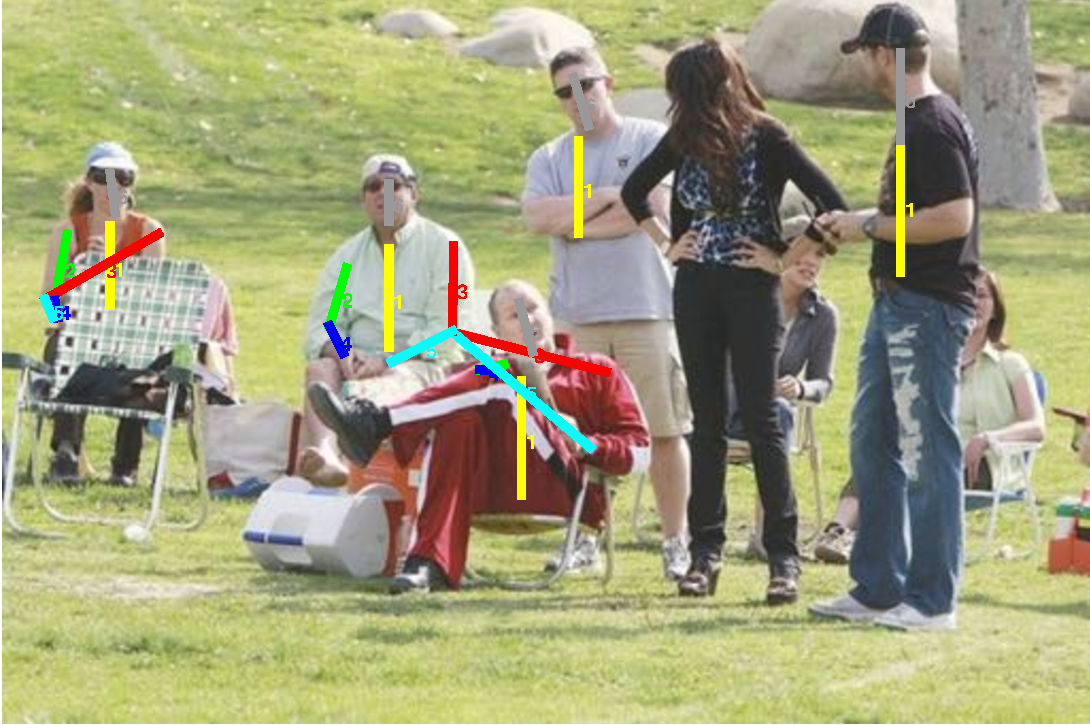
\includegraphics[height=0.275\linewidth]{imgidx_0028_sticks_unary_waf.pdf}\\
  %\includegraphics[height=0.275\linewidth]{imgidx_0001_sticks_waf.pdf}&
  %\includegraphics[height=0.275\linewidth]{imgidx_0001_sticks_unary_waf.pdf}\\
  %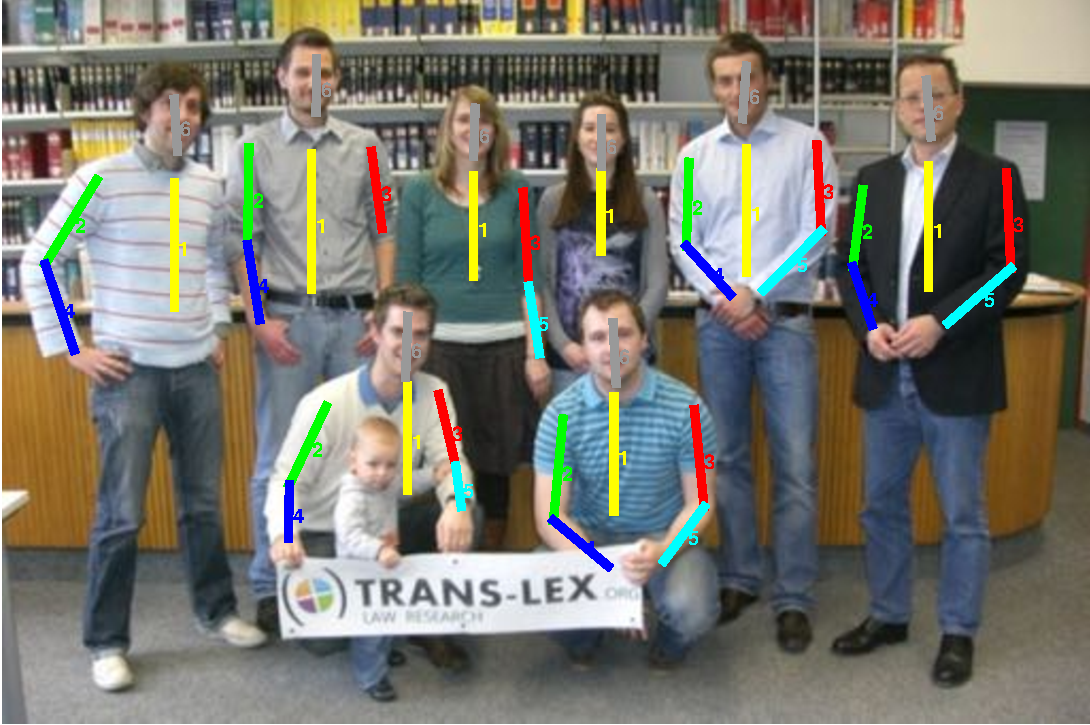
\includegraphics[height=0.275\linewidth]{imgidx_0124_sticks_waf.pdf}&
  %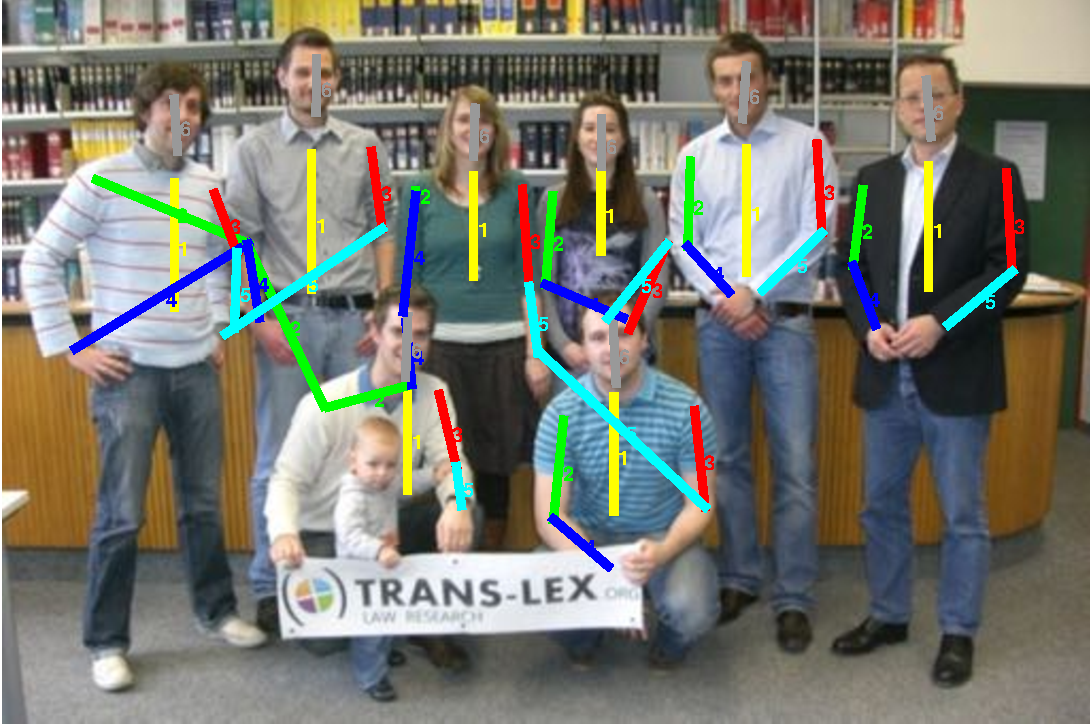
\includegraphics[height=0.275\linewidth]{imgidx_0124_sticks_unary_waf.pdf}\\
% \quad\quad\textbf{Chen\&Yuille}~\cite{Chen:2015:POC}
%\textbf{\deepcut~\multb~\dense} & \quad\textbf{\dense~\detroi}\\
  \end{tabular}
  %\vspace{-0.1em}
\caption{Qualitative comparison of our joint formulation
  $\deepcut~\multb~\dense$ (middle) to the traditional two-stage
  approach $\dense~\detroi$ (top) and the approach of
  Chen\&Yuille~\cite{Chen:2015:POC} (bottom) on WAF dataset. In
  contrast to $\detroi$, $\deepcut~\multb$ is able to disambiguate
  multiple and potentially overlapping persons and correctly assemble
  independent detections into plausible body part configurations. In
  contrast to ~\cite{Chen:2015:POC}, $\deepcut~\multb$ can better
  predict occlusions (image 2 person $1-4$ from the left, top row;
  image 4 person 1, 4; image 5, person 2) and better cope with strong
  articulations and foreshortenings (image 1, person 1, 3; image 2
  person 1 bottom row; image 3, person 1-2). See
  Appendix~\ref{sec:supplemental:waf} for more examples.
  %See supplementary material for more examples.
    %, but may fail                                                                                                                                                                                                                           
    %due to missing recall of part detection set (row 4 person 2, row 5                                                                                                                                                                       
    %person 3, 4).                                                                                                                                                                                                                            
  }
   \vspace{-1.0em}
  \label{fig:qualitative_waf_2}
\end{figure*}
